\section{Successioni}

\begin{definition}[Successione]
  Una successione in un dato insieme $X$ è una funzione $f:D\to X$ con dominio $D$ numerabile (il più delle volte $D\subseteq \mathbb{N}$). La si indica con $\left\{ x_n \right\}_{n\in D}\subseteq X$.
\end{definition}

\subsection{Limite}

\begin{definition}[Limite di successione]
  Una successione $\left\{ x_n \right\}_{n\in\mathbb{N}}\subseteq\mathbb{Q}$ converge al numero $\l\in\mathbb{Q}$, in simboli:
  $$\lim_{n\to+\infty} x_n=\l\ \mathrm{oppure}\ x_n\xrightarrow{n\to+\infty}\l$$
  se:
  $$\forall\epsilon>0\ \exists\ N\(\epsilon\)\in\mathbb{N}:n\ge N\(\epsilon\)\impl \abs{x_n-\l}<\epsilon$$
  cioè:
  $$\forall\epsilon>0\ \exists\ N\(\epsilon\)\in\mathbb{N}:n\ge N\(\epsilon\)\impl \l-\epsilon<x_n<\l+\epsilon$$
  cioè:
  $$\forall\epsilon>0\ \exists\ N\(\epsilon\)\in\mathbb{N}:n\ge N\(\epsilon\)\impl x_n\in\ointv{\l-\epsilon}{\l+\epsilon}$$
  \begin{center}
    \begin{tikzpicture}[scale=1.5]
      \draw[-stealth] (0,0) -- (6,0) node [right] {$\mathbb{Q}$};
      \draw (3,0) node [label=below:$\l$] {};
      \draw (3,0) circle (1.5pt);
      \draw (2.5,0) node [label=$x_n$] {};
      \fill (2.5,0) circle (1.5pt);
      \draw (2,0) node [label=below:$\l-\epsilon$] {$\vert$};
      \draw (4,0) node [label=below:$\l+\epsilon$] {$\vert$};
    \end{tikzpicture}
  \end{center}
\end{definition}

\begin{example}
  $$\lim_{n\to+\infty}\frac{1}{n}=0$$
  \begin{center}
    \begin{tikzpicture}[scale=5]
      \draw[-stealth] (-0.3,0) -- (1.3,0) node [right] {$\mathbb{Q}$};
      \draw (0,0) node [label=below:$0$] {$\vert$};
      \foreach \n in {1,...,5} {
          \draw (1/\n,0) node {$\vert$};
          \node[below=8pt] at (1/\n,0) {$\frac{1}{\n}$};
        }
    \end{tikzpicture}
  \end{center}
  Fissato $\epsilon>0$, si ha:
  $$0-\epsilon<\frac{1}{n}<0+\epsilon$$
  $$-\epsilon<\frac{1}{n}<\epsilon\iff \frac{1}{n}<\epsilon$$
  $$n>\frac{1}{\epsilon}$$
  Si sceglie $N\(\epsilon\)$ come il più piccolo numero naturale maggiore di $\nicefrac{1}{\epsilon}$, in modo tale da avere:
  $$n\ge N\(\epsilon\)>\frac{1}{\epsilon}$$
  e, quindi, verificare la definizione di limite.
\end{example}

\begin{example}
  $$\lim_{n\to+\infty}n=+\infty$$
  \begin{center}
    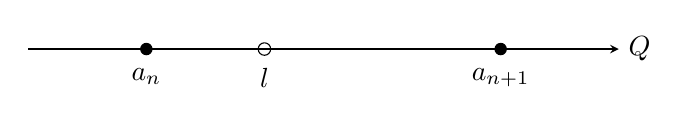
\begin{tikzpicture}[scale=1.5]
      \draw[-stealth] (0,0) -- (5,0) node [right] {$\mathbb{Q}$};
      \draw (1,0) node [label=below:$a_{n}$] {};
      \fill (1,0) circle (1.5pt);
      \draw (4,0) node [label=below:$a_{n+1}$] {};
      \fill (4,0) circle (1.5pt);
      \draw (2,0) node [label=below:$\l$] {};
      \draw (2,0) circle (1.5pt);
    \end{tikzpicture}
  \end{center}
  Si dice che la successione tende a $+\infty$, ossia il limite esiste ma non è un numero $\in\mathbb{Q}$.
\end{example}

\subsection{Proprietà}

\begin{lemma}
  Se $\exists \lim_{n\to+\infty}a_n\in\mathbb{Q}$, allora tale limite è unico.
\end{lemma}
\begin{proof}
  Siano $a_n\xrightarrow{n\to+\infty}\l_1$ e $a_n\xrightarrow{n\to+\infty}\l_2$. Si ha:
  $$\forall\epsilon>0\ \exists\ N_1\(\epsilon\)\in\mathbb{N}:n\ge N_1\(\epsilon\)\impl \abs{a_n-\l_1}<\epsilon$$
  $$\forall\epsilon>0\ \exists\ N_2\(\epsilon\)\in\mathbb{N}:n\ge N_2\(\epsilon\)\impl \abs{a_n-\l_2}<\epsilon$$
  Fissato $\epsilon>0$, se $n\ge N\(\epsilon\)\walrus\max\left\{ N_1\(\epsilon\),N_2\(\epsilon\) \right\}$, allora $n\ge N_1\(\epsilon\)\wedge n\ge N_2\(\epsilon\)$ e:
  $$0\le \abs{\l_1-\l_2}<\abs{\l_1-a_n+a_n-\l_2}\le\abs{\l_1-a_n}+\abs{a_n-\l_2}\le\epsilon+\epsilon=2\epsilon$$
  $$0\le\abs{\l_1-\l_2}\le2\epsilon\impl \abs{\l_1-\l_2}=0\iff \l_1=\l_2$$
\end{proof}
\begin{lemma}
  Se $\exists \lim_{n\to+\infty}a_n\in\mathbb{Q}$, allora $\left\{ a_n \right\}$ è limitata.
\end{lemma}
\begin{proof}
  $$\l\walrus\lim_{n\to+\infty}a_n$$
  $$\forall\epsilon>0\ \exists\ N\(\epsilon\)\in\mathbb{N}:n\ge N\(\epsilon\)\impl a_n\in\ointv{\l-\epsilon}{\l+\epsilon}$$
  Allora $\left\{ a_n \right\}_{n\ge N\(\epsilon\)}\subset \ointv{\l-\epsilon}{\l+\epsilon}$, ed è quindi limitata, e $\left\{ a_n \right\}_{n< N\(\epsilon\)}$ è limitata in quanto insieme finito. Quindi:
  $$\left\{ a_n \right\}_{n\ge0}=\left\{ a_n \right\}_{n< N\(\epsilon\)}\cup \left\{ a_n \right\}_{n\ge N\(\epsilon\)}$$
  è limitata, in poiché unione di insiemi limitati.
\end{proof}
\begin{lemma}
  $$
    \begin{cases}
      \exists\ \l_1\walrus\lim_{n\to+\infty}a_n \\
      \exists\ \l_2\walrus\lim_{n\to+\infty}b_n \\
    \end{cases}
    \impl
    \lim_{n\to+\infty}\(a_n+b_n\)=\lim_{n\to+\infty}a_n+\lim_{n\to+\infty}b_n
  $$
\end{lemma}
\begin{proof}
  Dalle ipotesi, si ha:
  $$0\le\abs{\(a_n+b_n\)-\(\l_1+\l_2\)}=\abs{\(a_n-\l_1\)-\(b_n-\l_2\)}\le\abs{a_n-\l_1}+\abs{b_n-\l_2}<\epsilon+\epsilon=2\epsilon$$
  Dato che si può scegliere $\epsilon$ arbitrariamente piccolo, si ha:
  $$\abs{\(a_n+b_n\)-\(\l_1+\l_2\)}=0\iff \(a_n+b_n\)-\(\l_1+\l_2\)=0\iff a_n+b_n=\l_1+\l_2$$
\end{proof}
\begin{lemma}
  $$
    \begin{cases}
      \exists\ \l_1\walrus\lim_{n\to+\infty}a_n \\
      \exists\ \l_2\walrus\lim_{n\to+\infty}b_n \\
    \end{cases}
    \impl
    \lim_{n\to+\infty}\(a_n\cdot b_n\)=\(\lim_{n\to+\infty}a_n\)\cdot\(\lim_{n\to+\infty}b_n\)
  $$
\end{lemma}
\begin{proof}
  Dalle ipotesi, si ha:
  \begin{align*}
    0 & \le \abs{a_nb_n-\l_1\l_2}                         \\
      & =\abs{a_nb_n-\l_1b_n+\l_1b_n-\l_1\l_2}            \\
      & =\abs{b_n\(a_n-\l_1\)+\l_1\(b_n-\l_2\)}           \\
      & \le\abs{b_n\(a_n-\l_1\)}+\abs{\l_1\(b_n-\l_2\)}   \\
      & =\abs{b_n}\abs{a_n-\l_1}+\abs{\l_1}\abs{b_n-\l_2} 
  \end{align*}
  Dato che $\left\{ b_n \right\}$ converge, allora è anche limitata, per cui:
  $$\exists\ M\ge0:\abs{b_n}<M\ \forall n\ge0$$
  Da cui:
  $$0\le \abs{a_nb_n-\l_1\l_2} \le M\abs{a_n-\l_1}+\abs{\l_1}\abs{b_n-\l_2}<M\epsilon+\abs{\l_1}\epsilon=\epsilon\(M+\abs{\l_1}\)$$
  Dato che si può scegliere $\epsilon$ arbitrariamente piccolo, si ha:
  $$\abs{a_nb_n-\l_1\l_2}=0\iff a_nb_n-\l_1\l_2=0\iff a_nb_n=\l_1\l_2$$
\end{proof}
\begin{lemma}
  $$\lim_{n\to+\infty}\frac{a_n}{b_n}=\frac{\lim_{n\to+\infty}a_n}{\lim_{n\to+\infty}b_n}$$
\end{lemma}

\begin{lemma}[Convergenza delle successioni costanti]
  Sia $\left\{ c \right\}$, con $c\in\mathbb{Q}$ fissato.
  $$\lim_{n\to+\infty} c=c$$
\end{lemma}
\begin{proof}
  $$\forall \epsilon>0\ \abs{a_n-\l}=\abs{c-c}=0<\epsilon$$
\end{proof}
\begin{observation}
  Se $\exists\ \l\walrus\lim_{n\to+\infty}a_n$, si verifica il seguente fenomeno:
  \begin{center}
    \begin{tikzpicture}[scale=1.5]
      \draw[-stealth] (0,0) -- (6,0) node [right] {$\mathbb{Q}$};
      \draw[dashdotted] (3,-.3) node [below] {$N\(\epsilon\)$} -- (3,3.3);
      \draw[] (0,1.5) node [left] {$\l$} -- (6,1.5);
      \draw[dashed] (0,0.9) node [left] {$\l-\epsilon$} -- (6,0.9);
      \draw[dashed] (0,2.1) node [left] {$\l+\epsilon$} -- (6,2.1);
      \foreach \i in {1,...,8} {
          \pgfmathrandominteger{\x}{1}{15}
          \fill (\i / 3,\x / 5) circle (1.5pt);
        }
      \foreach \i in {6,...,11} {
          \pgfmathrandominteger{\x}{1}{5}
          \fill (\i / 2,\x / 5 + 1) circle (1.5pt);
        }
    \end{tikzpicture}
  \end{center}
\end{observation}

\begin{example}
  \begin{align*}
    \lim_{n\to+\infty} \frac{n}{n+1} & =\lim_{n\to+\infty}\frac{n+1-1}{n+1}                               \\
                                     & =\lim_{n\to+\infty}\frac{n+1}{n+1}-\lim_{n\to+\infty}\frac{1}{n+1} \\
                                     & =\lim_{n\to+\infty}1-\lim_{n\to+\infty}\frac{1}{n+1}               \\
                                     & =1-0=1                                                             
  \end{align*}
\end{example}

\begin{theorem}[Permanenza del segno]
  $$a_n\ge0\wedge\exists\ \l\walrus\lim_{n\to+\infty}a_n\impl\l\ge0$$
\end{theorem}
\begin{proof}
  Per assurdo, sia $\l<0$. Sia $\epsilon\walrus-\nicefrac{\l}{2}>0$. Poiché esiste il limite, si ha:
  $$\exists\ N\(\epsilon\)\ge0:n\ge N\(\epsilon\)\impl \l-\epsilon<a_n<\l+\epsilon$$
  da cui:
  $$\l+\nicefrac{\l}{2}<a_n<\l-\nicefrac{\l}{2}$$
  $$\nicefrac{3}{2}\l<a_n<\nicefrac{1}{2}\l<0$$
  per cui si ha l'assurdo.
\end{proof}

\begin{theorem}[Monotonia]
  $$
    \begin{cases}
      a_n\le b_n                                \\
      \exists\ \l_1\walrus\lim_{n\to+\infty}a_n \\
      \exists\ \l_2\walrus\lim_{n\to+\infty}b_n \\
    \end{cases}
    \impl
    \l_1\le\l_2
  $$
\end{theorem}

\begin{theorem}
  $$\lim_{n\to+\infty}a_n=0\wedge \left\{ b_n \right\}\subseteq\ointv{a}{b}\impl\exists\ \lim_{n\to+\infty}a_nb_n=0$$  
\end{theorem}

\begin{definition}
  $$\lim_{n\to-\infty}a_n=\l\iff \forall\epsilon>0\ \exists\ N\(\epsilon\)\le0:n\le N\(\epsilon\)\impl\abs{a_n-\l}<\epsilon$$
\end{definition}

\begin{definition}
  $$\lim_{n\to+\infty}a_n=+\infty\iff \forall M\in\mathbb{Q}\ \exists\ N\(M\)\ge0:n\ge N\(M\)\impl a_n\ge M$$
\end{definition}

Tutte le proprietà dei limiti continuano a valere anche nel caso in cui $\left\{ a_n \right\}$ e $\left\{ b_n \right\}$ convergano a $\pm\infty$, tranne nei casi seguenti, detti di indecisione:
\begin{itemize}
  \item $+\infty-\infty$
  \item $0\cdot \infty$
  \item $\nicefrac{\infty}{\infty}$
  \item $\nicefrac{0}{0}$
\end{itemize}
Per convenzione $\infty\cdot\infty=\infty$.

\begin{example}
  $$a_n\walrus\(1+\frac{1}{n}\)^n$$
  \begin{align*}
    a_n & =\(1+\frac{1}{n}\)^n                                                               \\
        & =\sum_{k=0}^n\binom{n}{k}1^{n-k}\(\frac{1}{n}\)^k                                  \\
        & =\sum_{k=0}^n\frac{n!}{k!\(n-k\)!}\frac{1}{n^k}                                    \\
        & =\frac{n!}{0!n!n^0}+\frac{n!}{1!\(n-1\)!n^1}+\sum_{k=2}^n\frac{n!}{n^kk!\(n-k\)!}  \\
        & =2+\sum_{k=2}^n\frac{n\(n-1\)\cdots\(n-k+1\)\(n-k\)!}{n^kk!\(n-k\)!}               \\
        & =2+\sum_{k=2}^n\frac{n\(n-1\)\cdots\(n-k+1\)}{n^kk!}                               \\
        & =2+\sum_{k=2}^n\frac{1}{k!}\cdot\frac{n}{n}\cdot\frac{n-1}{n}\cdots\frac{n-k+1}{n} \\
        & =2+\sum_{k=2}^n\frac{1}{k!}\(1-\frac{1}{n}\)\cdots\(1-\frac{k-1}{n}\)              
  \end{align*}
  \begin{align*}
    a_{n+1} & =2+\sum_{k=2}^{n+1}\frac{1}{k!}\(1-\frac{1}{n+1}\)\cdots\(1-\frac{k-1}{n+1}\) \\
            & \ge2+\sum_{k=2}^{n}\frac{1}{k!}\(1-\frac{1}{n+1}\)\cdots\(1-\frac{k-1}{n+1}\) \\
            & \ge2+\sum_{k=2}^{n}\frac{1}{k!}\(1-\frac{1}{n}\)\cdots\(1-\frac{k-1}{n}\)     \\
            & =a_n                                                                          
  \end{align*}
  $$a_{n+1}\ge a_n$$
  Essendo crescente, $\left\{ a_n \right\}$ è inferiormente limitata:
  $$a_n\ge a_1=\(1+\frac{1}{1}\)^1=2$$
  Inoltre:
  \begin{align*}
    a_n & <2+\sum_{k=2}^n\frac{1}{k!}                           \\
        & \le 2+\sum_{k=2}^n\frac{1}{2^{k-1}}                   \\
        & =2+\sum_{k=0}^n\frac{1}{2^{k-1}}-2-1                  \\
        & =\sum_{k=0}^n\frac{1}{2^{k-1}}-1                      \\
        & =\sum_{k=0}^n\frac{2}{2^{k}}                          \\
        & =2\sum_{k=0}^n\frac{1}{2^k}-1                         \\
        & =2\(\frac{1-\(\frac{1}{2}\)^{n+1}}{1-\frac{1}{2}}\)-1 \\
        & =4\(1-\frac{1}{2^{n+1}}\)-1                           
  \end{align*}
  Passando al limite:
  $$
    \lim_na_n<\lim_n 4\(1-\frac{1}{2^{n+1}}\)-1 = 4-1=3
  $$
  In conclusione, $\forall n\ge1\ a_n\in\rintv{2}{3}$.
\end{example}

\subsection{Costruzione di $\reals$}

\begin{theorem}[Proprietà di Cauchy]
  Se $\exists\ \lim_{n}a_n\in\mathbb{Q}$, allora:
  $$\forall\epsilon>0\ \exists\ N\(\epsilon\)\ge0:n,m\ge N\(\epsilon\)\impl \abs{a_n-a_m}<\epsilon$$
\end{theorem}
\begin{proof}
  Sia $\l\walrus\lim_na_n$. Allora:
  $$\forall\epsilon>0\ \exists\ N\(\epsilon\)\ge0:n\ge N\(\epsilon\)\impl \abs{x_n-\l}<\epsilon$$
  Da cui, se $n,m\ge N\(\epsilon\)$:
  $$0\le\abs{a_n-a_m}=\abs{\(a_n-\l\)+\(\l-a_m\)}\le\abs{a_n-\l}+\abs{a_m-\l}\le 2\epsilon$$
  Perciò:
  $$\abs{a_n-a_m}<2\epsilon$$
\end{proof}


\begin{definition}[Relazione di equivalenza]
  Sia $X$ un insieme. Una \textbf{relazione di equivalenza} su $X$ è un insieme $R\subset X\times X$, avente le seguenti proprietà:
  \begin{itemize}
    \item riflessività: $\(x,x\)\in R\ \forall x\in X$ oppure $x\stackrel{R}{\sim}x$
    \item simmetria: $\(x,y\)\in R\impl \(y,x\)\in R$ oppure $x\stackrel{R}{\sim}y\impl y\stackrel{R}{\sim}x$
    \item transitività: $\(x,y\),\(y,z\)\in R\impl \(x,z\)\in R$ oppure $x\stackrel{R}{\sim}y\wedge y\stackrel{R}{\sim}z\impl x\stackrel{R}{\sim}z$
  \end{itemize}
\end{definition}

\begin{definition}[Insieme quoziente]
  Sia $\left[ x \right]_R\walrus\left\{ y\in X:x\stackrel{R}{\sim}y \right\}\subset X$. L'\textbf{insieme quozionte} è definito come:
  $$\nicefrac{X}{R}\walrus\left\{ \left[ x \right]_R:x\in X \right\}$$
\end{definition}

Sia $X\walrus\left\{ \text{successioni di Cauchy in }\mathbb{Q} \right\}$. Le successioni $\left\{ a_n \right\},\left\{ b_n \right\}$ sono in relazione $R$ se:
$$\lim_{n\to+\infty}\(a_n-b_n\)=0$$
Si dimostra che che $R$ è una relazione di equivalenza.

\begin{definition}[Numeri reali]
  L'insieme dei \textbf{numeri reali} è definito come:
  $$\reals\walrus \nicefrac{X}{R}$$
\end{definition}

Si definiscono le seguenti operazioni su $\reals$.

\begin{definition}[Somma in $\reals$]
  Siano $\left[ \left\{ a_n \right\} \right]_R,\left[ \left\{ b_n \right\} \right]_R\in\reals$. La loro somma è:
  $$\left[ \left\{ a_n \right\} \right]_R+\left[ \left\{ b_n \right\} \right]_R\walrus\left[ \left\{ a_n+b_n \right\} \right]_R$$
\end{definition}

\begin{definition}[Prodotto in $\reals$]
  Siano $\left[ \left\{ a_n \right\} \right]_R,\left[ \left\{ b_n \right\} \right]_R\in\reals$. Il loro prodotto è:
  $$\left[ \left\{ a_n \right\} \right]_R\cdot\left[ \left\{ b_n \right\} \right]_R\walrus\left[ \left\{ a_n\cdot b_n \right\} \right]_R$$
\end{definition}

\begin{observation}
  Queste operazioni godono delle ``solite'' proprietà: associatività, distributività, elementi neutri, etc...
\end{observation}

\begin{definition}[Positività]
  Si dirà che $\left[ \left\{ a_n \right\} \right]_R\in\reals$ è positivo se:
  $$\exists\ q>0\in\mathbb{Q},\exists\ N\ge0:n\ge N\impl a_n\ge q$$
\end{definition}

\begin{definition}[Ordine in $\reals$]
  Siano $\left[ \left\{ a_n \right\} \right]_R,\left[ \left\{ b_n \right\} \right]_R\in\reals$. Si stabilisce l'ordine:
  $$\left[ \left\{ a_n \right\} \right]_R<\left[ \left\{ b_n \right\} \right]_R\iff \left[ \left\{ b_n \right\} \right]_R-\left[ \left\{ a_n \right\} \right]_R>0$$
\end{definition}

\begin{observation}
  Si può ``immergere'' $\mathbb{Q}$ in $\reals$, poiché esiste una funzione iniettiva $j:\mathbb{Q}\to\reals$:
  $$j\(x\)\walrus\left[ \left\{ x \right\} \right]_R\in\reals$$
  $$j\(x\)+j\(y\)=j\(x+y\)$$
  $$j\(x\)\cdot j\(y\)=j\(x\cdot y\)$$
\end{observation}

\begin{definition}[Intervalli in $\reals$]
  Siano $a,b\in\reals:a<b$:
  \begin{itemize}
    \item l'insieme $\ointv{a}{b}\walrus\left\{ x\in\reals:a<x<b \right\}$ è detto \textbf{intervallo aperto};
    \item l'insieme $\intv{a}{b}\walrus\left\{ x\in\reals:a\le x\le b \right\}$ è detto \textbf{intervallo chiuso};
    \item l'insieme $\lintv{a}{b}\walrus\left\{ x\in\reals:a<x\le b \right\}$ è detto \textbf{intervallo semiaperto a sinistra};
    \item l'insieme $\rintv{a}{b}\walrus\left\{ x\in\reals:a\le x<b \right\}$ è detto \textbf{intervallo semiaperto a destra}.
  \end{itemize}
\end{definition}

\begin{definition}[Limite di successione]
  Una successione $\left\{ x_n \right\}\subseteq\reals$ converge al numero $\l\in\reals$, in simboli:
  $$\lim_{n\to+\infty} x_n=\l\ \mathrm{oppure}\ x_n\xrightarrow{n\to+\infty}\l$$
  se:
  $$\forall\epsilon>0\ \exists\ N\(\epsilon\)\in\mathbb{N}:n\ge N\(\epsilon\)\impl \abs{x_n-\l}<\epsilon$$
\end{definition}

\begin{observation}
  Tutte le proprietà dei limiti di successioni razionali restano valide anche per limiti di successioni di numeri reali.
\end{observation}

\begin{theorem}[Teorema fondamentale di completezza di $\reals$]
  La condizione di Cauchy per successioni di numeri reali è necessaria e sufficiente per la convergenza in $\reals$.
\end{theorem}

\begin{theorem}[Convergenza delle successioni monotone limitate]
  Sia $\left\{ x_n \right\}\subset\reals$ una successione monotona crescente e superiormente limitata:
  $$x_n\le x_{n+1}$$
  $$\exists\ M\in\reals:x_n\le M$$
  Allora $\left\{ x_n \right\}\subset\reals$ è di Cauchy e quindi convergente:
  $$\exists\ \lim_{n\to+\infty}x_n\in\reals$$
\end{theorem}
\begin{proof}
  Per la completezza di $\reals$ è sufficiente dimostrare che $\left\{ x_n \right\}$ è di Cauchy, ossia:
  $$\forall\epsilon>0\ \exists\ N\(\epsilon\)\ge1:n,m\ge N\(\epsilon\)\impl \abs{x_n-x_m}<\epsilon$$
  Per assurdo, se $\left\{ x_n \right\}$ non è di Cauchy, allora:
  $$\exists\epsilon>0\ \forall N\(\epsilon\)\ge1:\exists\ n,m\ge N\(\epsilon\)\impl \abs{x_n-x_m}\ge\epsilon$$
  Senza ledere la generalità della tesi, si assume che $x_n>x_m$. In questo modo:
  $$x_n-x_m=\abs{x_n-x_m}\ge\epsilon\iff x_n\ge\epsilon+x_m$$
  $$N\(\epsilon\)=1\impl\exists\ n_1>m_1:x_{n_1}\ge\epsilon+x_{m_1}$$
  $$N\(\epsilon\)=n_1\impl \exists\ n_2>m_2\ge N\(\epsilon\) \ge n_1 >m_1:x_{n_2}\ge\epsilon+x_{m_2}\ge\epsilon+x_{n_1}\ge 2\epsilon+x_{m_1}$$
  $$N\(\epsilon\)=n_k>m_k\impl\exists\ n_{k+1}>m_{k+1}\ge N\(\epsilon\)\ge n_k>m_k$$
  Per la monotonia del limite, si ha:
  $$\lim_{k\to+\infty}x_{n_{k+1}}\ge \lim_{k\to+\infty}k\epsilon+x_{m_1}=\epsilon\(+\infty\)+x_{m_1}=+\infty$$
  Ma ciò contraddice l'ipotesi di limitatezza della successione, per cui $\left\{ x_n \right\}$ è di Cauchy e pertanto converge in $\reals$.
\end{proof}

\begin{definition}[Maggiorante e minorante]
  Sia $A\subseteq\reals$.
  $x_0\in\reals$ è detto \textbf{maggiorante} di $A$ se $x\in A\impl x<x_0$.
  Analogamente, $x_0$ è detto \textbf{minorante} di $A$ se $x\in A\impl x>x_0$.
\end{definition}

\begin{definition}[Estremi superiore ed inferiore]
  Sia $A\subseteq\reals$.
  $x_0$ è detto \textbf{estremo superiore} di $A$, indicato con $\sup A$, se $x_0$ è maggiorante di $A$ ed è il suo più piccolo maggiorante, vale a dire che $\forall\epsilon>0\ x_0-\epsilon$ non è maggiorante di $A$.
  Analogamente, $x_0$ è detto \textbf{estremo inferiore} di $A$, indicato con $\inf A$, se $x_0$ è minorante di $A$ ed è il suo più grande minorante, vale a dire che $\forall\epsilon>0\ x_0+\epsilon$ non è minorante di $A$.
\end{definition}

\begin{definition}[Massimo e minimo]
  Sia $A\subseteq\reals$.
  Se $\sup A\in A$, allora $\sup A$ è detto \textbf{massimo} di $A$.
  Se $\inf A\in A$, allora $\inf A$ è detto \textbf{minimo} di $A$.
\end{definition}

\begin{theorem}[Esistenza di $\sup A$ e/o $\inf A$]
  Se $A\subseteq\reals$ è superiormente limitato, ossia ha almeno un maggiorante, allora $\exists\ \sup A\in\reals$.
\end{theorem}
\begin{proof}
  Poiché $A$ è superiormente limitato, $\exists\ b_0\in\reals:x\in A\impl x\le b_0$. Sia $a_0\in A:\intv{a_0}{b_0}\cap A\neq\emptyset$. Sia $c$ il punto medio dell'intervallo: $$c\walrus\frac{a_0+b_0}{2}$$
  In almeno uno degli intervalli $\intv{a_0}{c}$ e $\intv{c}{b_0}$ vi sono punti di $A$. Senza ledere la generalità della dimostrazione, si considera l'ultimo intervallo e lo si indica con $\intv{a_1}{b_1}$:
  $$\intv{a_1}{b_1}\subset\intv{a_0}{b_0}$$
  $$\intv{a_1}{b_1}\cap A\neq \emptyset$$
  $$x\in A\impl x\le b_1$$
  Iterando questo processo (che prende il nome di dicotomia), si ottiene una successione decrescente di intervalli:
  $$\intv{a_{n+1}}{b_{n+1}}\subset\intv{a_n}{b_n}\subset\cdots\subset\intv{a_0}{b_0}$$
  per cui si verifica che $\forall n\ge0\ b_n$ è un maggiorante di $A$.
  Si ha che $\left\{ a_n \right\}$ è crescente e superiormente limitata da $b_0$ e $\left\{ b_n \right\}$ è decrescente e inferiormente limitata da $a_0$.
  Per il teorema di convergenza delle successioni monotone limitate:
  $$\exists\ \lim_{n\to+\infty}a_n\quad\wedge\quad\exists\ \lim_{n\to+\infty}b_n$$
  Inoltre:
  $$\lim_{n\to+\infty}\(b_n-a_n\)=\lim_{n\to+\infty}\frac{b_0-a_0}{2^n}=0$$
  da cui:
  $$\reals\ni\bar{x}\walrus \lim_{n\to+\infty}a_n=\lim_{n\to+\infty}b_n$$
  $$\forall x\in A\impl x\le b_n$$
  $$\forall x\in A\impl \lim_{n\to+\infty}x\le \lim_{n\to+\infty}b_n$$
  $$\forall x\in A\impl x\le \bar{x}$$
  ossia $\bar{x}$ è un maggiorante di $A$.
  Sia $\epsilon>0$.
  $$\bar{x}=\lim_{n\to+\infty}a_n\impl\exists\ n\ge1:\bar{x}-\epsilon<a_n\le\bar{x}$$
  $$\intv{a_n}{b_n}\cap A\neq\emptyset\impl \exists\ x\in\intv{a_n}{b_n}\cap A\impl x\ge a_n$$
  $$\bar{x}-\epsilon<a_n\le x\le b_n$$
  pertanto $\bar{x}-\epsilon$ non è un maggiorante.
  Quindi $\bar{x}\in R$ è il più piccolo maggiorante, ossia $\bar{x}=\sup A$.
\end{proof}

\begin{definition}[Punti di accumulazione]
  Sia $E\subseteq\reals$. Un punto $\bar{x}\in\reals$ è detto \textbf{punto di accumulazione} di $E$ se:
  $$\forall\epsilon>0\ \(E\setminus\left\{ \bar{x} \right\}\)\cap\ointv{\bar{x}-\epsilon}{\bar{x}+\epsilon}\neq\emptyset$$
  ovvero:
  $$\forall\epsilon>0\ \exists\ x\in E:x\neq \bar{x}\wedge \abs{x-\bar{x}}<\epsilon$$
  ovvero:
  $$\forall\epsilon>0\ \#\(E\cap\ointv{\bar{x}-\epsilon}{\bar{x}+\epsilon}\)=+\infty$$
  Se $\bar{x}\in E$ non è di accumulazione, è detto \textbf{isolato}.
\end{definition}
\begin{observation}
  Non è detto che $\bar{x}\in E$.
\end{observation}

\begin{definition}[Insieme derivato]
  In generale, si denota con $E'$ l'insieme dei punti di accumulazione di $E$, detto \textbf{insieme derivato} di $E$.
\end{definition}

\begin{theorem}[Proprietà di Bolzano--Weierstrass]
  Sia $E\subseteq \reals$ limitato e infinito. Allora $\exists\ \bar{x}\in E'$.
\end{theorem}
\begin{proof}
  Poiché limitato, $E\subseteq\intv{a_0}{b_0}$. Sia $c$ il punto medio dell'intervallo:
  $$c\walrus\frac{a_0+b_0}{2}$$
  In almeno uno fra gli intervalli $\intv{a_0}{c}$ e $\intv{c}{b_0}$ vi sono infiniti punti di $E$, dato che $E\subseteq\intv{a_0}{b_0}=\intv{a_0}{c}\cup\intv{c}{b_0}$ e $\#\(E\)=+\infty$. Considerato tale intervallo, e indicandolo con $\intv{a_1}{b_1}$, si ha:
  $$\#\(E\cap\intv{a_1}{b_1}\)=+\infty$$
  Iterando la dicotomia, si ottiene una successione decrescente di intervalli:
  $$\intv{a_{n+1}}{b_{n+1}}\subset\intv{a_n}{b_n}\subset\cdots\subset\intv{a_0}{b_0}$$
  da cui:
  $$\#\(E\cap\intv{a_n}{b_n}\)=+\infty$$
  Si ha che $\left\{ a_n \right\}$ è crescente e superiormente limitata da $b_0$ e $\left\{ b_n \right\}$ è decrescente e inferiormente limitata da $a_0$.
  Per il teorema di convergenza delle successioni monotone limitate:
  $$\exists\ \lim_{n\to+\infty}a_n\quad\wedge\quad\exists\ \lim_{n\to+\infty}b_n$$
  Inoltre:
  $$\lim_{n\to+\infty}\(b_n-a_n\)=\lim_{n\to+\infty}\frac{b_0-a_0}{2^n}=0$$
  da cui:
  $$\reals\ni\bar{x}\walrus \lim_{n\to+\infty}a_n=\lim_{n\to+\infty}b_n$$
  Sia $x_n\in E\cap\intv{a_n}{b_n}:x_n\neq\bar{x}$. Si ha:
  $$a_n\le x_n\le b_n$$
  $$\bar{x}=\lim_{n\to+\infty}a_n\le \lim_{n\to+\infty}x_n\le \lim_{n\to+\infty}b_n=\bar{x}$$
  $$\bar{x}=\lim_{n\to+\infty}x_n$$
  Pertanto, $\bar{x}$ è di accumulazione per $E$: $$\bar{x}\in E'$$
\end{proof}
